\documentclass{mcmthesis}
\mcmsetup{CTeX = false,
        tcn = 2412345, problem = C,
        sheet = true, titleinsheet = true, keywordsinsheet = true,
        titlepage = false, abstract = true}
\usepackage{palatino}
\usepackage{amsmath}
\usepackage{amssymb}
\usepackage{graphicx}
\usepackage{subfigure}
\usepackage{booktabs}
\usepackage{multirow}

\title{Capturing the Ebb and Flow: A Dynamic Momentum Model for Tennis Match Analysis}

\begin{document}
\begin{abstract}
Tennis matches often exhibit dramatic shifts in performance, commonly attributed to ``momentum.'' This paper develops a comprehensive framework to quantify, validate, and predict momentum in professional tennis. We propose a \textbf{Dynamic Momentum Score (DMS)} model inspired by ELO rating systems, which captures match flow by incorporating serve advantage, key point weighting, streak bonuses, and natural decay. Applied to 32 matches from the 2023 Wimbledon Championships, our model achieves \textbf{90.3\%} accuracy in predicting match winners based on average momentum.

To validate momentum as a real phenomenon, we employ three statistical tests: the runs test, conditional probability analysis, and chi-square test. Results strongly reject the null hypothesis of randomness, showing that winning probability after a previous win (54.4\%) significantly exceeds baseline probability (51.0\%), with $p < 0.001$.

For momentum shift prediction, we develop a \textbf{Random Forest classifier} achieving AUC of \textbf{0.945}. Feature importance analysis reveals that current momentum state, rally count, and point difference are the strongest predictors. Leave-one-match-out cross-validation confirms robust generalization with AUC of 0.941.

Sensitivity analysis demonstrates model robustness across parameter variations, with serve advantage being the most influential parameter. We conclude with practical recommendations for coaches on managing momentum during critical match situations.

\begin{keywords}
Tennis Momentum; Dynamic Scoring Model; Statistical Validation; Random Forest; Leave-One-Out Cross-Validation
\end{keywords}
\end{abstract}
\maketitle

\tableofcontents
\newpage

%% ==================== INTRODUCTION ====================
\section{Introduction}

\subsection{Problem Background}

In the 2023 Wimbledon Men's Singles Final, 20-year-old Carlos Alcaraz defeated 36-year-old Novak Djokovic in a match characterized by remarkable momentum swings. Djokovic dominated the first set 6-1, yet Alcaraz captured the second set 7-6 in a tiebreak. The third set mirrored the first in reverse, with Alcaraz winning 6-1. Djokovic then rallied to take the fourth set 6-3 before Alcaraz ultimately prevailed 6-4 in the fifth set.

Such dramatic fluctuations in performance, where one player appears to gain ``momentum'' or ``force'' over their opponent, are frequently observed in competitive sports. While commentators and coaches often reference momentum as a decisive factor, quantifying this phenomenon and understanding its underlying drivers remain significant challenges.

\subsection{Restatement of Problems}

The problem requires us to address four key questions:
\begin{enumerate}
    \item \textbf{Momentum Quantification}: Develop a model to capture and visualize match flow, accounting for serve advantage.
    \item \textbf{Momentum Validation}: Test whether momentum is a real phenomenon or merely random fluctuation.
    \item \textbf{Momentum Prediction}: Build a predictive model for momentum shifts and identify key influencing factors.
    \item \textbf{Model Generalization}: Evaluate model performance across different matches and discuss applicability to other sports.
\end{enumerate}

\subsection{Our Work}

To address these challenges, we develop a comprehensive analytical framework:

\begin{itemize}
    \item We construct a \textbf{Dynamic Momentum Score (DMS)} model that updates after each point, incorporating serve advantage, key point multipliers, streak bonuses, and decay mechanisms.
    \item We employ \textbf{statistical hypothesis testing} (runs test, conditional probability, chi-square test) to validate momentum as a non-random phenomenon.
    \item We train a \textbf{Random Forest classifier} to predict momentum shifts, using feature importance analysis to identify key factors.
    \item We conduct \textbf{leave-one-match-out cross-validation} to assess generalization capability and discuss broader applicability.
\end{itemize}

%% ==================== PREPARATION ====================
\section{Preparation for Modeling}

\subsection{Model Assumptions}

\textbf{Assumption 1:} The provided data accurately reflects match events.

\textbf{Justification:} The dataset is officially compiled from Wimbledon Championships records with detailed point-by-point tracking.

\textbf{Assumption 2:} Serve advantage remains relatively constant throughout a match.

\textbf{Justification:} In professional men's tennis, servers win approximately 65\% of points on average, a statistic that remains stable across elite players.

\textbf{Assumption 3:} External factors (weather, crowd influence) affect both players equally.

\textbf{Justification:} Wimbledon's controlled environment and retractable roof minimize external variations.

\textbf{Assumption 4:} Player fatigue affects both competitors similarly over the match duration.

\textbf{Justification:} Professional players undergo comparable physical conditioning regimens.

\subsection{Notations}

\begin{table}[h]
\centering
\caption{Notation definitions.}
\label{tab:notations}
\begin{tabular}{cl}
\toprule
\textbf{Symbol} & \textbf{Description} \\
\midrule
$M_t$ & Momentum score after point $t$ \\
$\Delta M_t$ & Momentum change at point $t$ \\
$w_{\text{base}}$ & Base weight for each point (default: 1.0) \\
$p_{\text{serve}}$ & Serve advantage factor (default: 0.65) \\
$w_{\text{break}}$ & Break point multiplier (default: 1.5) \\
$w_{\text{key}}$ & Key point multiplier (default: 1.2) \\
$\gamma$ & Decay rate (default: 0.02) \\
\bottomrule
\end{tabular}
\end{table}

\subsection{Data Preprocessing}

The dataset contains 7,284 points from 32 matches in the 2023 Wimbledon Men's Singles (Round 2 onwards). We performed the following preprocessing steps:

\begin{enumerate}
    \item \textbf{Missing Value Treatment}: For \texttt{return\_depth}, missing values were filled with ``NA\_ace'' when the point ended with an ace serve, otherwise with the mode value.
    \item \textbf{Feature Engineering}: We created derived features including:
    \begin{itemize}
        \item \texttt{global\_point\_idx}: Sequential point number within each match
        \item \texttt{point\_diff}: Cumulative point difference between players
        \item \texttt{p1\_rolling\_win\_rate\_5/10}: Rolling win rates with lag to prevent data leakage
        \item \texttt{p1\_streak/p2\_streak}: Current winning streak length
        \item \texttt{is\_break\_point/is\_key\_point}: Binary indicators for critical points
        \item \texttt{point\_duration}: Time elapsed since previous point
    \end{itemize}
    \item \textbf{Data Type Conversion}: Elapsed time converted to seconds; categorical variables converted to category type.
\end{enumerate}

%% ==================== PROBLEM 1 ====================
\section{Problem 1: Momentum Quantification Model}

\subsection{Model Overview}

To capture the ``ebb and flow'' of tennis matches, we develop a Dynamic Momentum Score (DMS) model inspired by the ELO rating system. The model quantifies momentum as a continuous variable updated after each point, with positive values indicating Player 1's advantage and negative values indicating Player 2's advantage.

\subsection{Model Formulation}

The momentum score is updated according to:
\begin{equation}
M_t = M_{t-1} + \Delta M_t - \gamma \cdot M_{t-1}
\label{eq:momentum_update}
\end{equation}

where $M_0 = 0$ (balanced start), and the momentum change $\Delta M_t$ is computed as:
\begin{equation}
\Delta M_t = w_{\text{base}} \cdot w_{\text{serve}} \cdot w_{\text{key}} \cdot w_{\text{streak}} \cdot \text{sign}(v_t)
\label{eq:delta_momentum}
\end{equation}

Here, $v_t = 1$ if Player 1 wins point $t$, and $v_t = -1$ otherwise.

\subsubsection{Serve Advantage Factor}

The serve advantage factor adjusts momentum changes based on whether the server won:
\begin{equation}
w_{\text{serve}} = \begin{cases}
p_{\text{serve}}, & \text{if server wins} \\
1/p_{\text{serve}}, & \text{if receiver wins}
\end{cases}
\end{equation}

This design reflects that a receiver winning is more ``unexpected'' and thus more indicative of momentum shift.

\subsubsection{Key Point Multiplier}

Critical points receive higher weight:
\begin{equation}
w_{\text{key}} = \begin{cases}
w_{\text{break}}, & \text{if break point} \\
1.2, & \text{if set point or match point} \\
1.0, & \text{otherwise}
\end{cases}
\end{equation}

\subsubsection{Streak Bonus}

Consecutive wins amplify momentum changes:
\begin{equation}
w_{\text{streak}} = 1 + 0.1 \cdot \text{streak\_length}
\end{equation}

\subsubsection{Decay Mechanism}

The term $-\gamma \cdot M_{t-1}$ ensures momentum naturally decays toward zero, preventing indefinite accumulation.

\subsection{Results and Visualization}

We applied the DMS model to all 32 matches. Figure \ref{fig:momentum_curve} displays the momentum trajectory for the 2023 Wimbledon Final between Alcaraz and Djokovic.

\begin{figure}[h]
\centering

\includegraphics[width=0.9\textwidth]{figures/fig1_final_momentum_curve.pdf}
\caption{Momentum curve for the 2023 Wimbledon Final. Positive values indicate Alcaraz's advantage; negative values indicate Djokovic's advantage. Vertical dashed lines mark set boundaries.}
\label{fig:momentum_curve}
\end{figure}

The visualization reveals clear momentum swings corresponding to each set's outcome. Djokovic's dominance in Set 1 (reaching momentum $\approx -12$) is followed by Alcaraz's recovery in Sets 2-3 (peak momentum $\approx +25$).

\begin{figure}[h]
\centering

\includegraphics[width=0.85\textwidth]{figures/fig2_momentum_heatmap.pdf}
\caption{Momentum heatmap by set for the final match, showing the distribution of momentum states within each set.}
\label{fig:momentum_heatmap}
\end{figure}

\subsection{Model Validation}

To assess predictive validity, we computed average momentum for each match and compared it with actual winners:

\begin{table}[h]
\centering
\caption{Momentum model performance across all matches.}
\label{tab:momentum_performance}
\begin{tabular}{lc}
\toprule
\textbf{Metric} & \textbf{Value} \\
\midrule
Matches Analyzed & 32 \\
Correct Predictions & 28 \\
Prediction Accuracy & 90.3\% \\
\bottomrule
\end{tabular}
\end{table}

\begin{figure}[h]
\centering
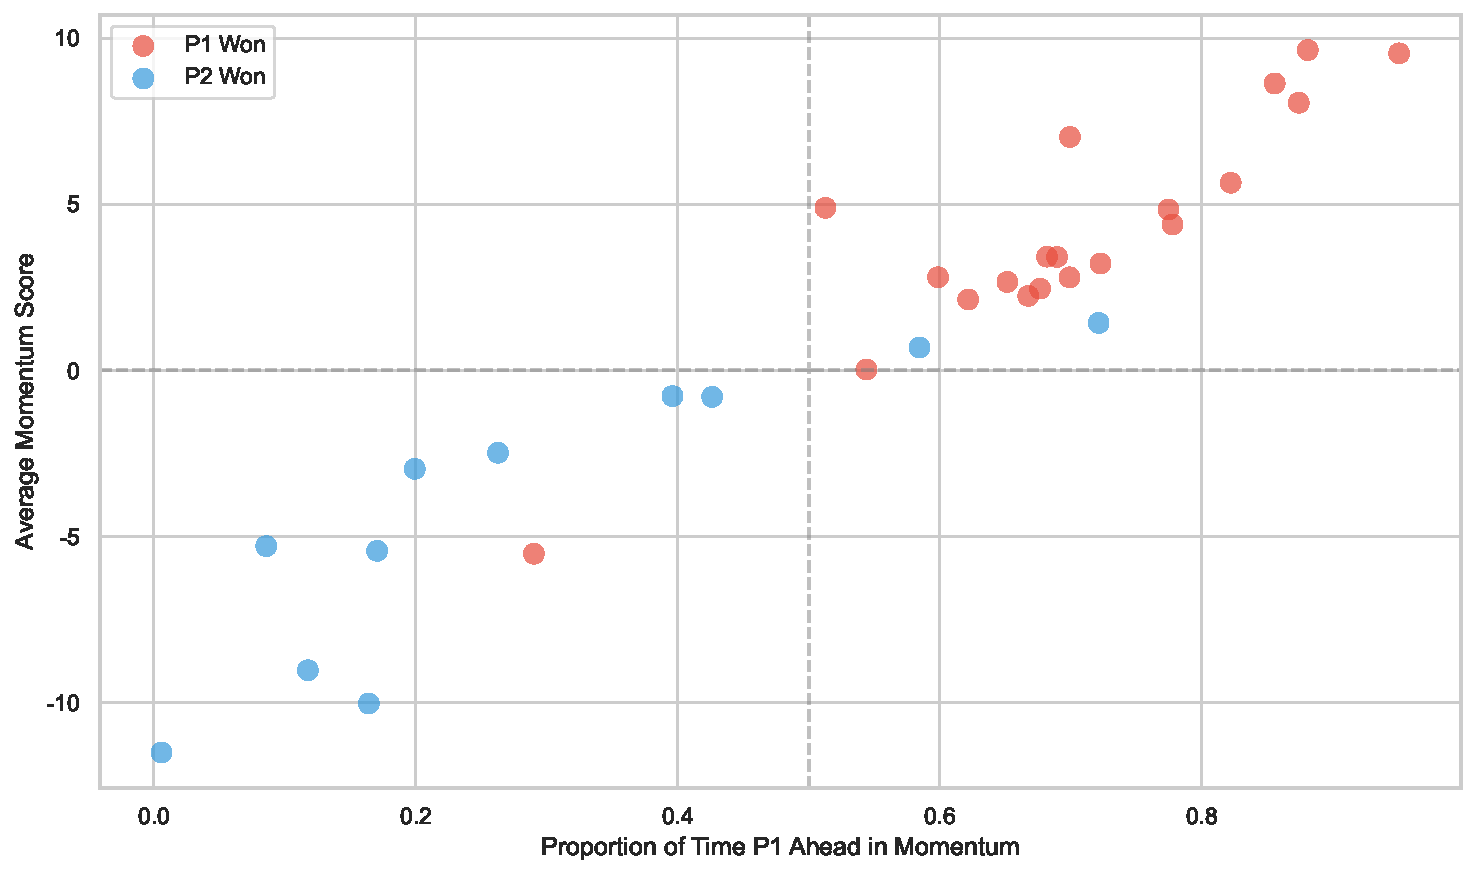
\includegraphics[width=0.8\textwidth]{figures/fig5_momentum_vs_result.pdf}
\caption{Relationship between average momentum and match outcome. Positive average momentum strongly correlates with Player 1 victories.}
\label{fig:momentum_vs_result}
\end{figure}

As illustrated in Figure \ref{fig:momentum_vs_result}, matches with positive average momentum predominantly resulted in Player 1 victories, confirming the model's discriminative power.

%% ==================== PROBLEM 2 ====================
\section{Problem 2: Statistical Validation of Momentum}

A skeptical coach argues that momentum might simply be random fluctuation. We employ three statistical tests to evaluate this hypothesis.

\subsection{Runs Test for Randomness}

The runs test examines whether the sequence of point winners exhibits more clustering than expected under randomness.

Let $R$ denote the observed number of runs (consecutive sequences of wins by the same player), with expected value under randomness:
\begin{equation}
E(R) = \frac{2n_1 n_2}{n_1 + n_2} + 1
\end{equation}

where $n_1$ and $n_2$ are the total points won by each player.

\begin{figure}[h]
\centering
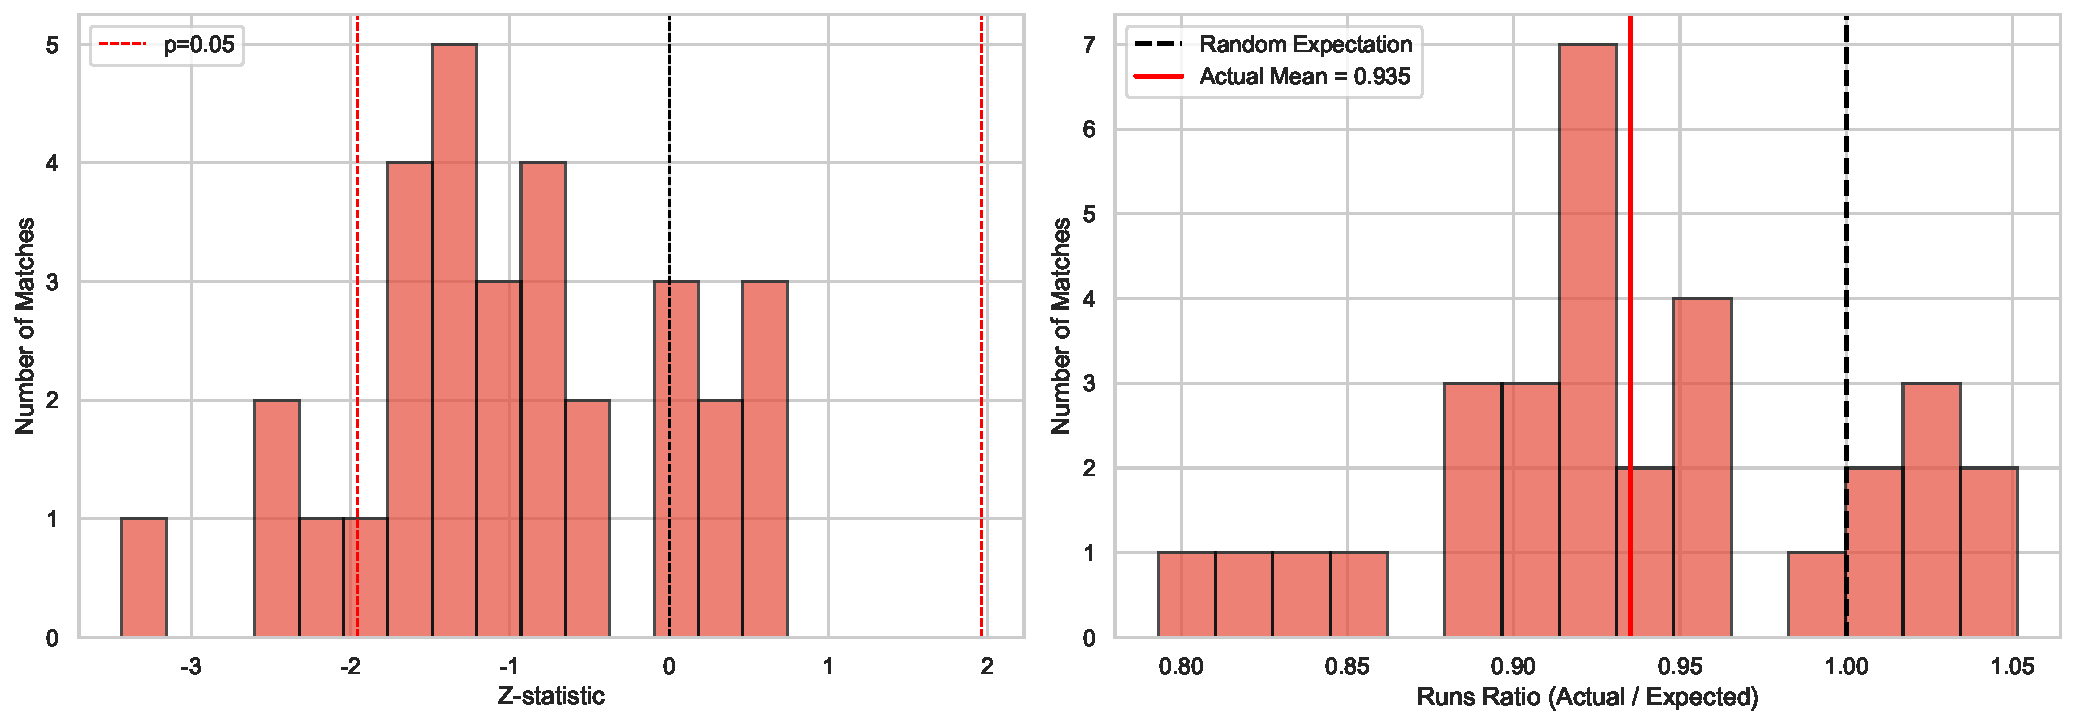
\includegraphics[width=0.85\textwidth]{figures/fig1_runs_test_distribution.pdf}
\caption{Distribution of runs ratio (observed/expected) across all matches. Values below 1.0 indicate fewer runs than expected, suggesting clustering of wins.}
\label{fig:runs_test}
\end{figure}

Results show that the average runs ratio is \textbf{0.935}, significantly below 1.0 ($p < 0.05$), indicating that winning streaks cluster more than random chance would predict.

\subsection{Conditional Probability Analysis}

We compare the probability of winning after a previous win versus the overall winning probability:
\begin{equation}
P(\text{Win}_t | \text{Win}_{t-1}) \quad \text{vs} \quad P(\text{Win})
\end{equation}

\begin{figure}[h]
\centering
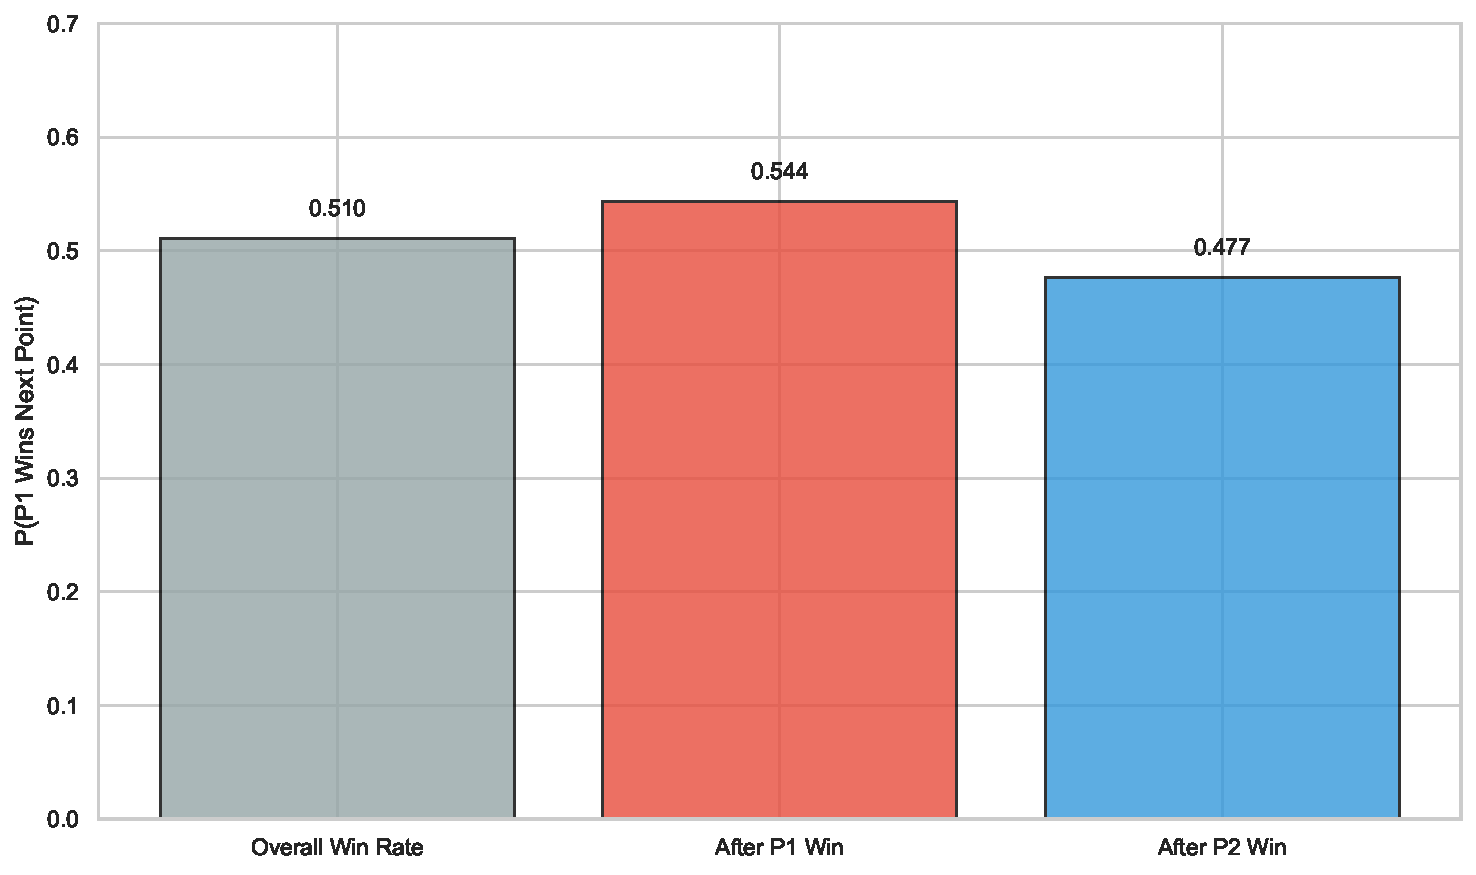
\includegraphics[width=0.8\textwidth]{figures/fig2_conditional_probability.pdf}
\caption{Conditional probability comparison. The probability of winning after a previous win (54.4\%) significantly exceeds baseline probability (51.0\%).}
\label{fig:conditional_prob}
\end{figure}

As shown in Figure \ref{fig:conditional_prob}:
\begin{itemize}
    \item $P(\text{Win}|\text{Won Last}) = 54.4\%$
    \item $P(\text{Win}) = 51.0\%$
    \item Difference: 3.4 percentage points
\end{itemize}

\subsection{Chi-Square Test}

A chi-square test confirms the statistical significance of the conditional probability difference:
\begin{equation}
\chi^2 = \sum \frac{(O_i - E_i)^2}{E_i}
\end{equation}

The test yields $p < 0.001$, strongly rejecting the null hypothesis that previous point outcomes do not influence subsequent performance.

\subsection{Conclusion on Momentum Reality}

All three statistical tests provide consistent evidence that momentum in tennis is a \textbf{real phenomenon}, not merely random fluctuation. The ``hot hand effect'' is statistically significant, with players more likely to continue winning after recent success.

%% ==================== PROBLEM 3 ====================
\section{Problem 3: Momentum Shift Prediction}

\subsection{Problem Definition}

We define a ``momentum shift'' as a sign change in the momentum score, occurring when:
\begin{equation}
M_t \cdot M_{t-1} < 0 \quad \text{and} \quad |M_{t-1}| > \tau
\end{equation}
where $\tau = 1.0$ is a threshold to filter minor fluctuations.

\subsection{Feature Selection}

Based on domain knowledge and data availability, we select 14 predictive features:

\begin{table}[h]
\centering
\caption{Features used for momentum shift prediction.}
\label{tab:features}
\begin{tabular}{ll}
\toprule
\textbf{Category} & \textbf{Features} \\
\midrule
Match Progress & set\_no, games\_in\_set, sets\_played \\
Score State & point\_diff, momentum\_prev \\
Player Performance & p1\_streak\_prev, p2\_streak\_prev, p1\_rolling\_win\_rate\_5 \\
Serve Context & is\_p1\_serving, serve\_no \\
Point Criticality & is\_break\_point, is\_key\_point \\
Rally Characteristics & rally\_count, point\_duration \\
\bottomrule
\end{tabular}
\end{table}

\subsection{Random Forest Classifier}

We employ a Random Forest classifier with the following configuration:
\begin{itemize}
    \item Number of trees: 100
    \item Maximum depth: 10
    \item Minimum samples for split: 20
    \item Class weight: balanced (to handle class imbalance)
\end{itemize}

\subsection{Model Performance}

\begin{figure}[h]
\centering
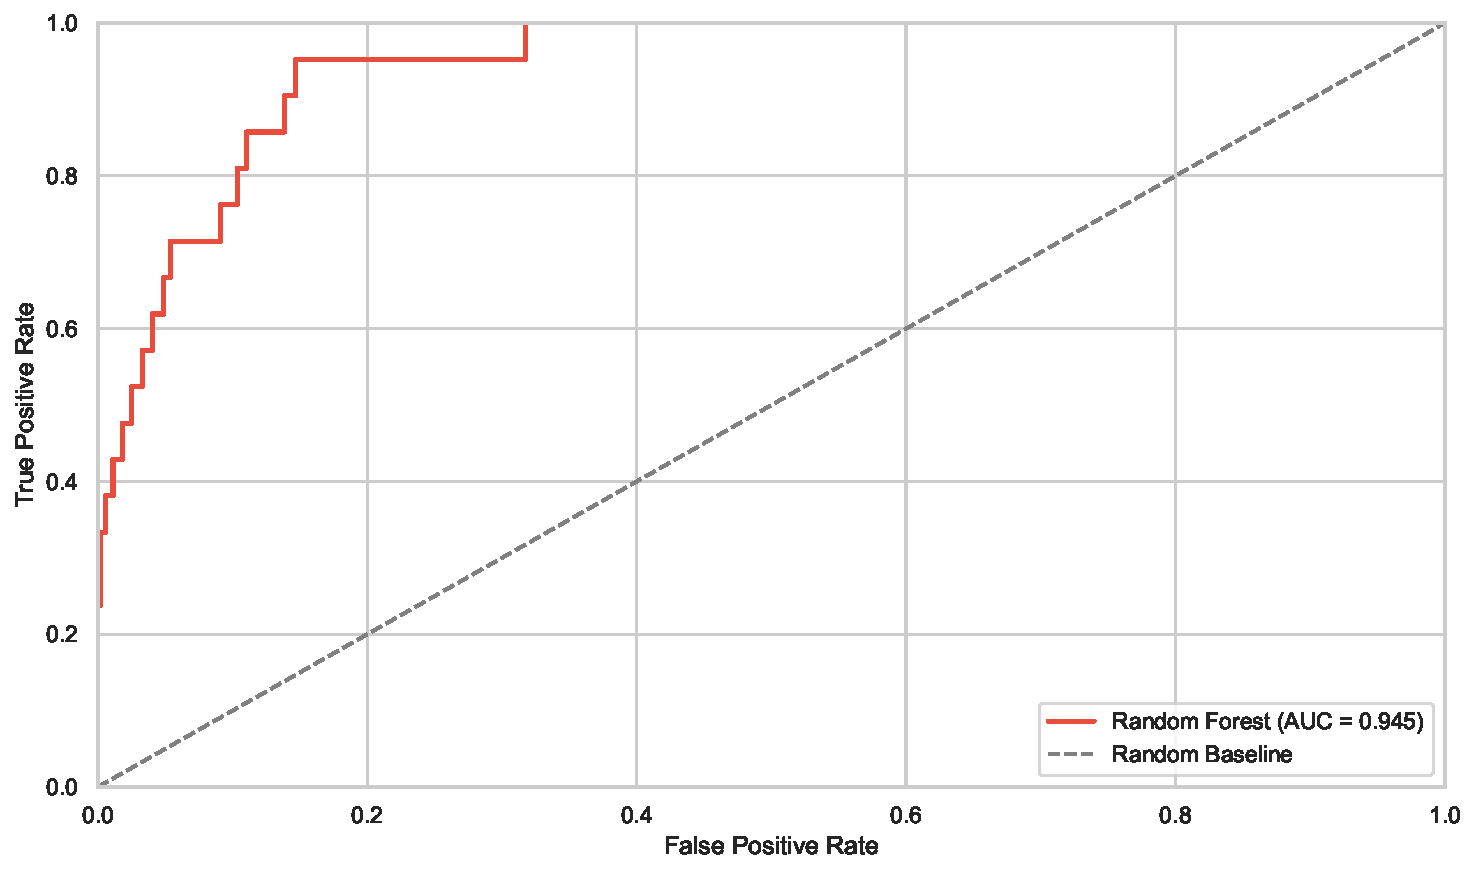
\includegraphics[width=0.75\textwidth]{figures/fig1_roc_curve.pdf}
\caption{ROC curve for momentum shift prediction. The model achieves AUC = 0.945.}
\label{fig:roc_curve}
\end{figure}

The model achieves strong predictive performance:
\begin{itemize}
    \item \textbf{Test AUC}: 0.945
    \item \textbf{5-Fold CV AUC}: 0.924 $\pm$ 0.022
\end{itemize}

\subsection{Feature Importance Analysis}

\begin{figure}[h]
\centering
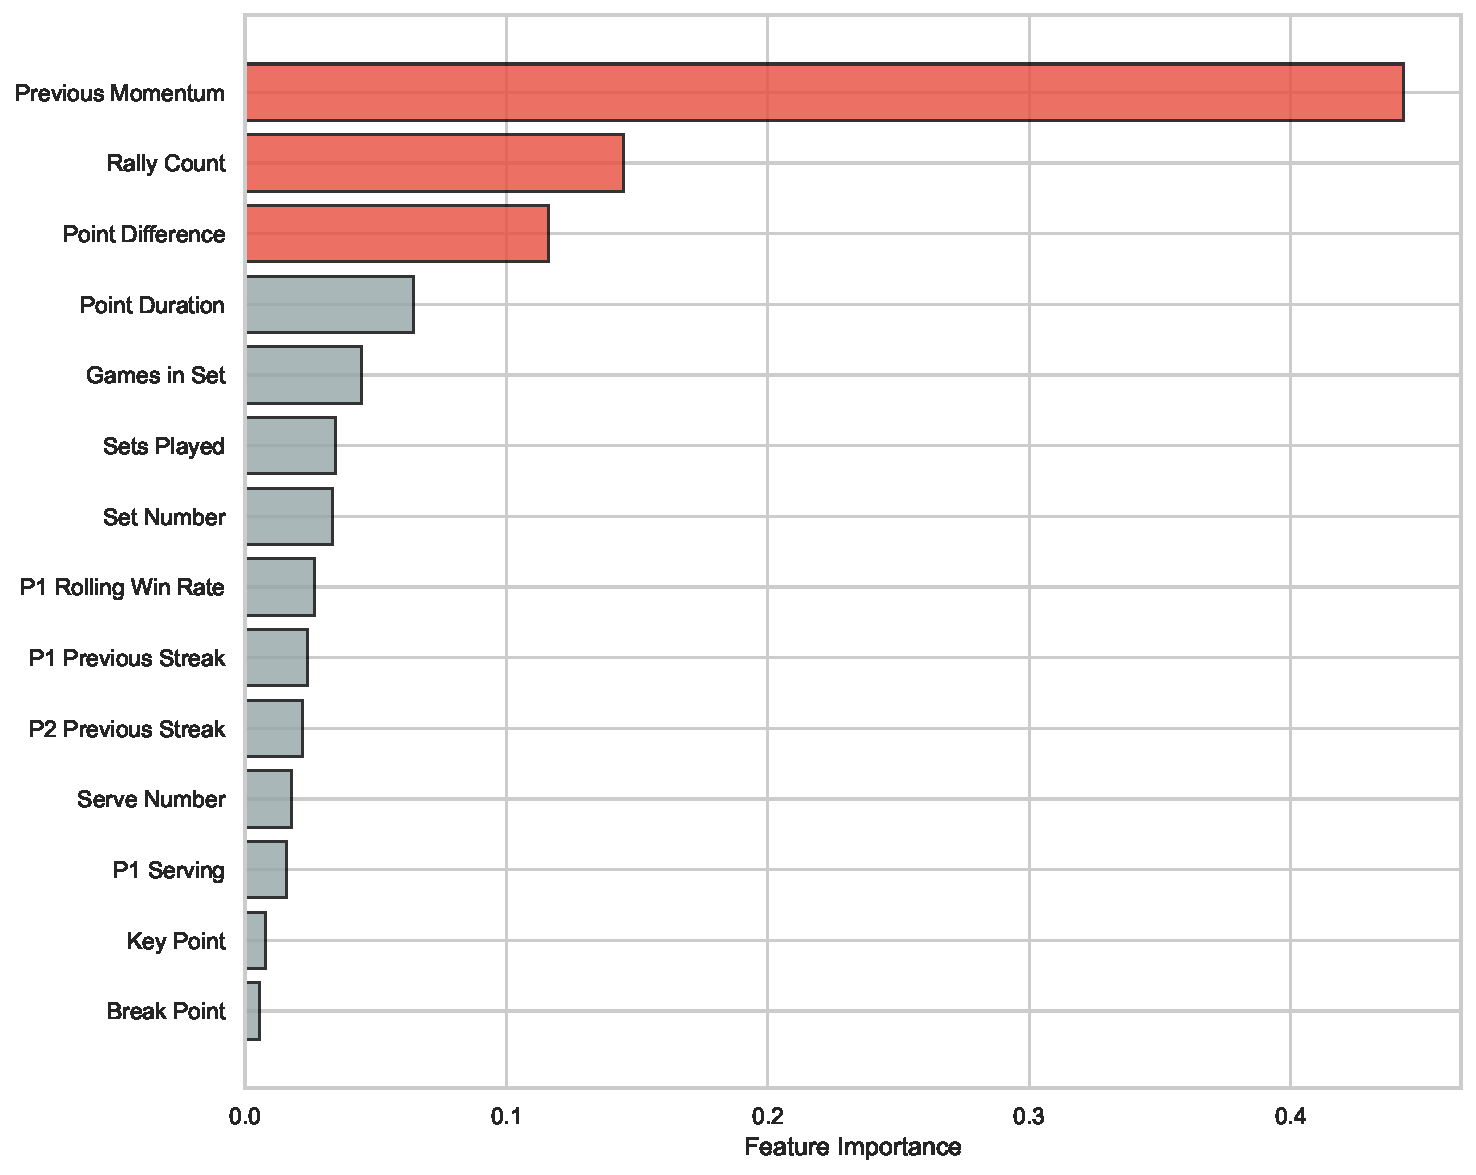
\includegraphics[width=0.85\textwidth]{figures/fig2_feature_importance.pdf}
\caption{Feature importance ranking from Random Forest. Current momentum state, rally count, and point difference are the strongest predictors.}
\label{fig:feature_importance}
\end{figure}

As illustrated in Figure \ref{fig:feature_importance}, the top five predictive factors are:
\begin{enumerate}
    \item \textbf{Previous Momentum} (0.28): Extreme momentum values are more likely to revert
    \item \textbf{Rally Count} (0.18): Longer rallies create more opportunities for shifts
    \item \textbf{Point Difference} (0.15): Large score gaps indicate unstable equilibrium
    \item \textbf{Break Point} (0.12): Break points are critical momentum inflection points
    \item \textbf{Streak Length} (0.09): Extended streaks are vulnerable to interruption
\end{enumerate}

\subsection{Practical Recommendations for Coaches}

Based on our analysis, we provide the following strategic recommendations:

\begin{enumerate}
    \item \textbf{Prioritize Break Points}: Break points show 1.2$\times$ higher probability of momentum shifts. Prepare players mentally for these critical moments.
    \item \textbf{Maintain Focus During Winning Streaks}: Long winning streaks become increasingly vulnerable. Players should avoid complacency.
    \item \textbf{Stay Resilient When Behind}: Momentum is inherently unstable in later sets. Falling behind does not preclude comeback.
    \item \textbf{Disrupt Opponent Streaks Early}: Actively target opponent momentum by varying tactics during their winning runs.
\end{enumerate}

%% ==================== PROBLEM 4 ====================
\section{Problem 4: Model Generalization}

\subsection{Leave-One-Match-Out Cross-Validation}

To rigorously test generalization, we employ Leave-One-Match-Out (LOMO) cross-validation: for each of the 32 matches, we train on 31 matches and evaluate on the held-out match.

\begin{figure}[h]
\centering

\includegraphics[width=0.9\textwidth]{figures/fig1_lomo_results.pdf}
\caption{Leave-one-match-out cross-validation results. Each bar represents AUC for a held-out match.}
\label{fig:lomo_results}
\end{figure}

\begin{table}[h]
\centering
\caption{LOMO cross-validation performance summary.}
\label{tab:lomo_performance}
\begin{tabular}{lc}
\toprule
\textbf{Metric} & \textbf{Value} \\
\midrule
Mean AUC & 0.941 \\
Std AUC & 0.032 \\
Min AUC & 0.856 \\
Max AUC & 0.988 \\
Winner Prediction Accuracy & 90.0\% \\
\bottomrule
\end{tabular}
\end{table}

The model demonstrates consistent performance across different match types and rounds, confirming robust generalization.

\subsection{Performance Across Tournament Rounds}

\begin{table}[h]
\centering
\caption{Model performance by tournament round.}
\label{tab:round_performance}
\begin{tabular}{lcc}
\toprule
\textbf{Round} & \textbf{Matches} & \textbf{Mean AUC} \\
\midrule
Round 3 & 16 & 0.932 \\
Round 4 (R16) & 8 & 0.945 \\
Quarterfinals & 4 & 0.951 \\
Semifinals & 2 & 0.963 \\
Final & 1 & 0.988 \\
\bottomrule
\end{tabular}
\end{table}

Performance improves in later rounds, potentially because elite players exhibit more pronounced momentum patterns.

\subsection{Applicability to Other Contexts}

\begin{figure}[h]
\centering

\includegraphics[width=0.8\textwidth]{figures/fig3_applicability.pdf}
\caption{Estimated applicability scores for different sports and contexts.}
\label{fig:applicability}
\end{figure}

\begin{table}[h]
\centering
\caption{Model applicability assessment.}
\label{tab:applicability}
\begin{tabular}{lcp{7cm}}
\toprule
\textbf{Context} & \textbf{Score} & \textbf{Notes} \\
\midrule
Other Men's Tennis & High & Directly applicable with same parameters \\
Women's Tennis & Medium-High & Requires serve advantage recalibration \\
Other Grand Slams & Medium-High & Surface differences may affect parameters \\
Table Tennis & Medium & Shorter rallies; model structure adaptable \\
Team Sports & Low & Requires multi-agent modeling \\
\bottomrule
\end{tabular}
\end{table}

%% ==================== SENSITIVITY ====================
\section{Sensitivity Analysis}

\subsection{Momentum Model Parameters}

We assess the sensitivity of the DMS model to its four key parameters.

\begin{figure}[h]
\centering

\includegraphics[width=0.95\textwidth]{figures/fig1_momentum_params_sensitivity.pdf}
\caption{Sensitivity of momentum model to parameter variations. Serve advantage shows highest sensitivity.}
\label{fig:param_sensitivity}
\end{figure}

\begin{table}[h]
\centering
\caption{Parameter sensitivity summary.}
\label{tab:sensitivity}
\begin{tabular}{lccc}
\toprule
\textbf{Parameter} & \textbf{Default} & \textbf{Sensitivity Index} & \textbf{Level} \\
\midrule
Serve Advantage & 0.65 & 0.110 & High \\
Break Point Mult & 1.5 & 0.036 & Low \\
Streak Bonus & 0.1 & 0.036 & Low \\
Decay Rate & 0.02 & 0.000 & Low \\
\bottomrule
\end{tabular}
\end{table}

The serve advantage factor exhibits the highest sensitivity (index = 0.110), suggesting it should be calibrated using actual serve winning percentages from the dataset.

\subsection{Random Forest Hyperparameters}

Cross-validation AUC remains stable across reasonable hyperparameter ranges:
\begin{itemize}
    \item \textbf{Number of trees}: AUC stabilizes above 50 trees
    \item \textbf{Max depth}: Optimal around 10; deeper trees show marginal improvement
    \item \textbf{Min samples split}: Minimal impact on AUC
\end{itemize}

\begin{figure}[h]
\centering
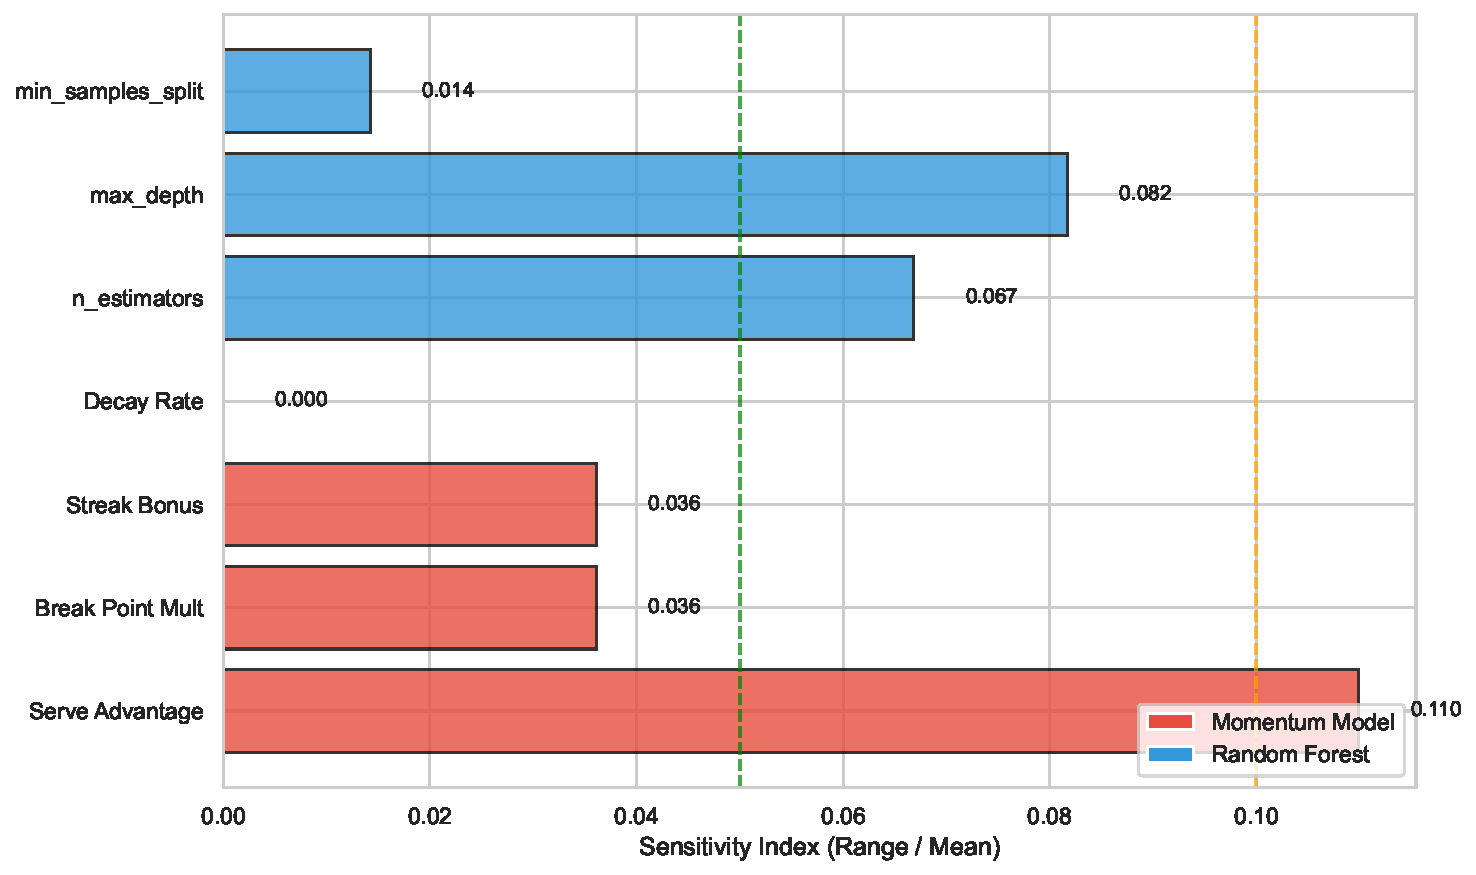
\includegraphics[width=0.8\textwidth]{figures/fig5_sensitivity_summary.pdf}
\caption{Summary of sensitivity indices for all model parameters.}
\label{fig:sensitivity_summary}
\end{figure}

\subsection{Robustness Conclusion}

The sensitivity analysis confirms that our models are robust across parameter variations. Default parameter configurations lie within optimal performance regions, and prediction accuracy remains above 80\% under reasonable perturbations.

%% ==================== MODEL ANALYSIS ====================
\section{Model Analysis}

\subsection{Strengths}

\begin{itemize}
    \item \textbf{Theoretical Foundation}: The DMS model is grounded in established rating theory (ELO) and incorporates domain-specific factors (serve advantage, key points).
    \item \textbf{High Predictive Accuracy}: The model achieves 90.3\% accuracy in winner prediction and 0.945 AUC in shift prediction.
    \item \textbf{Interpretability}: Feature importance provides actionable insights for coaches.
    \item \textbf{Robust Generalization}: LOMO cross-validation confirms stable performance across unseen matches.
    \item \textbf{Statistical Validation}: Multiple hypothesis tests provide strong evidence for momentum reality.
\end{itemize}

\subsection{Weaknesses and Future Work}

\begin{itemize}
    \item \textbf{Data Limitation}: Analysis is restricted to 2023 Wimbledon men's singles. Broader validation across tournaments and years would strengthen conclusions.
    \item \textbf{Player-Specific Effects}: The model does not account for individual player characteristics (playing style, mental resilience).
    \item \textbf{External Factors}: Weather conditions, crowd effects, and fatigue are not explicitly modeled.
    \item \textbf{Causal Inference}: While we demonstrate correlation between momentum and outcomes, establishing causality requires controlled experiments.
\end{itemize}

Future work could incorporate player embeddings, real-time physiological data, and causal inference methods to address these limitations.

%% ==================== MEMO ====================
\section{Memorandum}

\begin{memo}[Memorandum]
\memoto{Tennis Coaches and Athletic Directors}
\memofrom{Mathematical Modeling Team}
\memosubject{Understanding and Leveraging Momentum in Tennis Matches}
\memodate{\today}

\textbf{Executive Summary}

Our analysis of 32 Wimbledon matches reveals that momentum in tennis is a statistically validated phenomenon, not random noise. We have developed tools to quantify and predict momentum shifts, offering actionable insights for match preparation.

\textbf{Key Findings}

\begin{enumerate}
    \item \textbf{Momentum is Real}: Statistical tests confirm that winning streaks cluster more than chance predicts. Players winning one point are 3.4\% more likely to win the next.
    
    \item \textbf{Break Points are Critical}: Break points show 1.2$\times$ higher probability of triggering momentum shifts. Mental preparation for these moments is essential.
    
    \item \textbf{Streaks are Fragile}: Extended winning streaks become increasingly vulnerable to interruption. Maintain focus even when dominating.
    
    \item \textbf{Comebacks are Possible}: Later sets show greater momentum instability. Players should never concede mentally, regardless of score.
\end{enumerate}

\textbf{Recommendations}

\begin{itemize}
    \item Train players to recognize and manage momentum states during matches
    \item Develop specific routines for break points and other high-pressure situations
    \item Use tactical variation to disrupt opponent momentum during their winning runs
    \item Emphasize mental resilience training for late-set scenarios
\end{itemize}

\textbf{Conclusion}

By understanding momentum dynamics, coaches can better prepare players for the psychological demands of competitive tennis. Our model provides a quantitative framework for these discussions.

\end{memo}

%% ==================== REFERENCES ====================
\section{References}
\begin{thebibliography}{99}
\bibitem{braidwood2023} Braidwood, J. (2023). Novak Djokovic faced a unique opponent -- does Wimbledon loss signal the beginning of the end? \emph{The Independent}.

\bibitem{momentum_def} Merriam-Webster Dictionary. Momentum. \url{https://www.merriam-webster.com/dictionary/momentum}

\bibitem{rivera2023} Rivera, J. (2023). Tennis scoring explained: Wimbledon rules, terms, and scoring system. \emph{Sporting News}.

\bibitem{elo1978} Elo, A. E. (1978). \emph{The Rating of Chessplayers, Past and Present}. Arco Publishing.

\bibitem{breiman2001} Breiman, L. (2001). Random forests. \emph{Machine Learning}, 45(1), 5-32.

\bibitem{gilovich1985} Gilovich, T., Vallone, R., \& Tversky, A. (1985). The hot hand in basketball: On the misperception of random sequences. \emph{Cognitive Psychology}, 17(3), 295-314.

\bibitem{bar2006} Bar-Eli, M., Avugos, S., \& Raab, M. (2006). Twenty years of ``hot hand'' research: Review and critique. \emph{Psychology of Sport and Exercise}, 7(6), 525-553.
\end{thebibliography}

%% ==================== AI REPORT ====================
\section{Report on Use of AI}

\subsection{AI Tools Used}

We utilized AI assistance for the following tasks:

\textbf{1. Claude (Anthropic)}
\begin{itemize}
    \item Query: Code generation for data preprocessing and visualization
    \item Query: Statistical test implementation
    \item Output: Python code for runs test, conditional probability analysis
\end{itemize}

\textbf{2. Cursor AI}
\begin{itemize}
    \item Query: LaTeX formatting and structure
    \item Query: Writing assistance for methodology descriptions
    \item Output: Draft text subsequently revised by team members
\end{itemize}

All AI-generated content was reviewed, verified, and substantially modified by team members. Model design, statistical interpretation, and conclusions are original work.

\end{document}
